\documentclass{article}
\usepackage{bm}
\usepackage{amsmath}
\usepackage{graphicx}
\usepackage{mdwlist}
\usepackage[colorlinks=true]{hyperref}
\usepackage{geometry}
\usepackage{kotex}
\geometry{margin=1in}
\geometry{headheight=2in}
\geometry{top=2in}
\usepackage{palatino}
%\renewcommand{\rmdefault}{palatino}
\usepackage{fancyhdr}

%\pagestyle{fancy}
\rhead{}
\lhead{}
\chead{%
  {\vbox{%
      \vspace{2mm}
      \large
      Hardware System Design 4190.309A\hfill
\\
      Seoul National University
      \\[4mm]
      \textbf{Practice \#5. PE implementation \& BRAM modeling}\\
      \textbf{Jiwon Lee, Sangjun Son}
    }
  }
}

%%%%%%%%%%%%%%%%%%%%%%%
\usepackage{xcolor}
\usepackage{listings}
\definecolor{vgreen}{RGB}{104,180,104}
\definecolor{vblue}{RGB}{49,49,255}
\definecolor{vorange}{RGB}{255,143,102}

\lstdefinestyle{verilog-style}
{
    language=Verilog,
    basicstyle=\scriptsize\ttfamily,
    keywordstyle=\color{vblue},
    identifierstyle=\color{black},
    commentstyle=\color{vgreen},
    numbers=left,
    numberstyle=\tiny\color{black},
    numbersep=10pt,
    tabsize=8,
    moredelim=*[s][\colorIndex]{[}{]},
    literate=*{:}{:}1
}

\makeatletter
\newcommand*\@lbracket{[}
\newcommand*\@rbracket{]}
\newcommand*\@colon{:}
\newcommand*\colorIndex{%
    \edef\@temp{\the\lst@token}%
    \ifx\@temp\@lbracket \color{black}%
    \else\ifx\@temp\@rbracket \color{black}%
    \else\ifx\@temp\@colon \color{black}%
    \else \color{vorange}%
    \fi\fi\fi
}
\makeatother

\usepackage{trace}
%%%%%%%%%%%%%%%%%%%%%%%

\usepackage{paralist}

\usepackage{todonotes}
\setlength{\marginparwidth}{2.15cm}

\usepackage{tikz}
\usetikzlibrary{positioning,shapes,backgrounds}

\begin{document}

\pagestyle{fancy}

\section*{Goal}

\begin{itemize*}
\item Implement BRAM model \& test bench according to scenarios.
\begin{itemize*}
\item Make test bench that instantiates two BRAMs and initialize one BRAM to store address as data.
\item Copy every data from the initialized BRAM to the other BRAM.
\end{itemize*}
\item Implement PE with floating point fused multiply adder.
\end{itemize*}

\section{Implementation}

이번 프로젝트는 Block Random Access Memory와 Processing Element를 각각 구현함으로써 추후 구현할 Matrix-Matrix Multiplication을 수행하기 위한 기본 모듈을 구성하는 것을 목적으로 한다. 아래는 코드 구현과 함께 간략한 아이디어 및 기능에 대한 설명이 (1) BRAM, (2) PE 순으로 진행된다.

\subsection{Block Random Access Memory, BRAM}
BRAM의 경우 크게 두 부분으로 이뤄져 있다. (1) 모듈이 실행이 되기 전 INIT\_FILE에서 내부 메모리 \texttt{mem}를 읽는 부분과 done 신호가 주어졌을 때, OUT\_FILE에 \texttt{mem}의 상태를 출력하는 부분과, (2) EN, RST, WE 신호가 들어왔을 때 경우에 따라 입력되는 데이터를 \texttt{mem}에 읽고 쓰는 역할을 한다.

\begin{itemize*}
\item 아래에 첨부된 코드 중 21-28 라인의 외부 파일 입출력에 관한 구현 보면, \texttt{initial} 구문을 이용하여 모듈의 생성과 동시에 파일 입출력에 대한 실행 구문에 대한 scope를 지정한다. 
\texttt{\$readmemh} 로 시작함으로써 INIT\_FILE 파일을 읽어 \texttt{mem}에 저장한다. 
그 후 \texttt{done} 신호 들어올 때 까지 대기하다가 신호가 들어오면 \texttt{\$writememh} 함수를 사용해 OUT\_FILE에 \texttt{mem} 데이터를 저장한다.
이 때 함수에 붙어있는 \texttt{\$readmem\textbf{h}}와 \texttt{\$writemem\textbf{h}}의 \textbf{h}는 hexadecimal로 파일에 저장하는 값을 16진수 형태로 저장하는 옵션을 의미한다. \\
\item 30-46 라인은 BRAM의 input으로 주어지는 신호에 따라 모듈로써의 기능을 구현하는 부분이다. BRAM\_CLK와 BRAM\_RST 그리고 BRAM\_EN, BRAM\_WE의 신호에 따라 읽기, 쓰기, 초기화, 파일 출력을 위한 기능을 수행하게 된다. BRAM\_RST은 BRAM\_CLK에 Async로, BRAM\_EN, BRAM\_WE는 Sync로 구현하였다.
\begin{itemize*}
\item BRAM\_RST이 posedge일 경우 BRAM\_RDDATA에는 0을 할당한다. (31 라인)
\item BRAM\_EN이 활성화되어 있고 BRAM\_WE 또한 활성화되어 있다면, True를 가지는 bit에 해당하는 영역을 BRAM\_WRDATA에서 \texttt{mem}으로 복사한다. (35-38 라인)
\begin{equation}
\texttt{mem}[ \texttt{addr} ][8*(i+1)-1:8* i ]  \leftarrow \text{BRAM\_WRDATA}[8*(i+1) -1:8* i ] 
\end{equation}
\item BRAM\_EN이 활성화되어 있고 BRAM\_WE이 활성화되어 있다면, 메모리로부터 데이터를 읽어오는 기능을 수행한다. Read에 걸리는 싸이클이 2 cycle이 걸리도록 구현을 해야하기 때문에 \texttt{dout}을 버퍼로 사용해 1 cycle이 추가되도록 한다. (41-42 라인)
\end{itemize*}
\end{itemize*}

\subsubsection*{\texttt{MY\_BRAM}}
\begin{lstlisting}[style={verilog-style}]
`timescale 1ns / 1ps
module my_bram #(
    parameter integer BRAM_ADDR_WIDTH = 15,
    parameter INIT_FILE = "input.txt",
    parameter OUT_FILE = "output.txt"
)(
    input wire [BRAM_ADDR_WIDTH-1:0] BRAM_ADDR,
    input wire BRAM_CLK,
    input wire [31:0] BRAM_WRDATA,
    output reg [31:0] BRAM_RDDATA,
    input wire BRAM_EN,
    input wire BRAM_RST,
    input wire [3:0] BRAM_WE,
    input wire done
);
    reg [31:0] mem[0:8191];
    wire [BRAM_ADDR_WIDTH-3:0] addr = BRAM_ADDR[BRAM_ADDR_WIDTH-1:2];
    reg [31:0] dout;
    
    initial begin
        if (INIT_FILE != "") begin
            $readmemh(INIT_FILE, mem);
        end
        wait (done) begin
            $writememh(OUT_FILE, mem);
        end
    end
    
    always @(posedge BRAM_CLK or posedge BRAM_RST) begin
        if (BRAM_RST) begin 
            BRAM_RDDATA <= 0;
        end
        if (BRAM_EN) begin
            if (BRAM_WE) begin
                if (BRAM_WE[0]) mem[addr][7:0] <= BRAM_WRDATA[7:0];
                if (BRAM_WE[1]) mem[addr][15:8] <= BRAM_WRDATA[15:8];
                if (BRAM_WE[2]) mem[addr][23:16] <= BRAM_WRDATA[23:16];
                if (BRAM_WE[3]) mem[addr][31:24] <= BRAM_WRDATA[31:24]; 
            end
            else begin
                dout <= mem[addr];
                BRAM_RDDATA <= dout;
            end
        end
    end
endmodule
\end{lstlisting}

\newpage
\subsection{Processing Element, PE}

아래의 모듈은 Lab03 adder 모듈이다. ain과 bin 길이의 입력값이 

\subsubsection*{\texttt{MY\_PE}}
\begin{lstlisting}[style={verilog-style}]
`timescale 1ns / 1ps
module my_add #(
    parameter BITWIDTH = 32
)
(
    input [BITWIDTH-1:0] ain,
    input [BITWIDTH-1:0] bin,
    output [BITWIDTH-1:0] dout,
    output overflow
);
    // concatnate (overflow, dout) & detect overflow
    assign {overflow, dout} = ain + bin;
endmodule
\end{lstlisting}


\newpage
\section{Result}

\subsection{Block Random Access Memory, BRAM}
아래의 코드는 BRAM의 구현의 Validity를 확인하기 위해 시나리오에 맞게 구현한 것이다. BRAM 인스턴스 두 개를 만들고 각각을 MY\_BRAM1과 MY\_BRAM2로 명명하였다. 

MY\_BRAM1은 \texttt{input.txt}에 저장된 \texttt{mem}에 있는 값들을 호출하여 저장하는 역할을 하고 또한 \texttt{mem}에 있는 값들을 MY\_ADDR을 변화하면서 BRAM\_RDDATA1로 읽어온다. MY\_BRAM2의 경우 이렇게 읽어온 \linebreak BRAM\_RDDATA1을 BRAM\_WRDATA2로 사용하여 \texttt{mem}에 저장하게 되고 완료가 되면 \texttt{done} 신호를 주어 \linebreak \texttt{output.txt}에 저장하게 된다. 아래 Figure~\ref{fig1}은 상기된 설명을 도식화한 것이다.
\begin{figure}[ht]
	\centering
	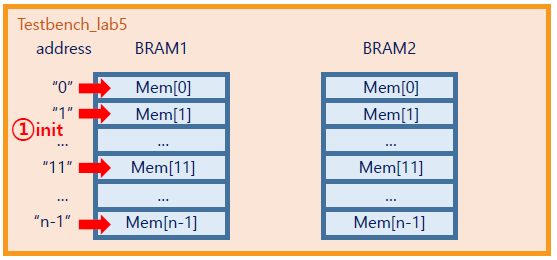
\includegraphics[width=0.49\textwidth]{fig/fig1.png}
	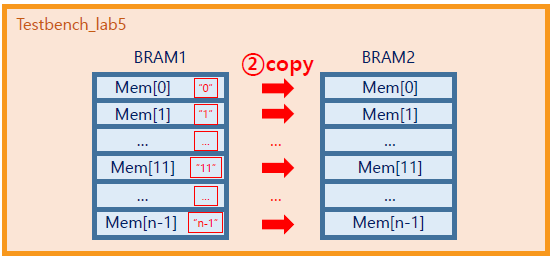
\includegraphics[width=0.49\textwidth]{fig/fig2.png}
\caption{Testbench Scenarios: 2개의 BRAM을 인스턴스화 하고 BRAM1에서 \texttt{input.txt}을 읽어 메모리에 저장하고 다른 BRAM2에서 BRAM1의 데이터를 전달받아  \texttt{output.txt}에 저장한다. }
\label{fig1}
\end{figure}

모든 테스트를 시작하기 전에 \texttt{input.txt}를 초기화하기 위한 과정을 거친다. 주소에 해당하는 인덱스를 값으로 가질 수 있도록 for문을 통해 대입시킨 후 \texttt{\$writememh}를 통해 파일에 저장을 한다. (23-24 라인)

\subsubsection*{\texttt{TB\_MY\_BRAM}}
\begin{lstlisting}[style={verilog-style}]
`timescale 1ns / 1ps

module tb_my_bram #(
    parameter integer BRAM_ADDR_WIDTH = 15,
    parameter INIT_FILE = "input.txt"
)();
    reg [31:0] BRAM_INIT[0:8191];
    reg [BRAM_ADDR_WIDTH-1:0] BRAM_ADDR;
    reg BRAM_CLK;
    reg BRAM_RST;
    reg [3:0] BRAM_WE;
    reg done;
    wire [31:0] BRAM_WRDATA1, BRAM_RDDATA1;
    wire [31:0] BRAM_WRDATA2, BRAM_RDDATA2;
    integer i;
    
    initial begin
        BRAM_ADDR <= 0;
        BRAM_CLK <= 1;
        BRAM_RST <= 0;
        BRAM_WE <= 0;
        done <= 0;
        for (i = 0; i < 8192; i = i + 1) begin
            BRAM_INIT[i][31:0] <= i;
        end
        #10 $writememh(INIT_FILE, BRAM_INIT);
        
        for (i = 0; i <= 8192; i = i + 1) begin
            BRAM_ADDR <= i << 2; #20;
            BRAM_WE <= 4'b1111; #10;
            BRAM_WE <= 0; #30;
        end
        done <= 1'b1; #30;
        BRAM_RST <= 1'b1;
    end
    
    always #5 BRAM_CLK = ~BRAM_CLK;
    assign BRAM_WRDATA2 = BRAM_RDDATA1;
    
    my_bram MY_BRAM1 (
        .BRAM_ADDR(BRAM_ADDR),
        .BRAM_CLK(BRAM_CLK),
        .BRAM_WRDATA(BRAM_WRDATA1),
        .BRAM_RDDATA(BRAM_RDDATA1),
        .BRAM_EN(1'b1),
        .BRAM_RST(BRAM_RST),
        .BRAM_WE(0),
        .done(0)
    );
    my_bram #(.INIT_FILE("")) MY_BRAM2 (
        .BRAM_ADDR(BRAM_ADDR),
        .BRAM_CLK(BRAM_CLK),
        .BRAM_WRDATA(BRAM_WRDATA2),
        .BRAM_RDDATA(BRAM_RDDATA2),
        .BRAM_EN(1'b1),
        .BRAM_RST(BRAM_RST),
        .BRAM_WE(BRAM_WE),
        .done(done)
    );
endmodule
\end{lstlisting}

위 Testbench 코드를 수행하면 아래와 같은 Waveform을 확인할 수 있다.
\begin{figure}[ht]
	\centering
	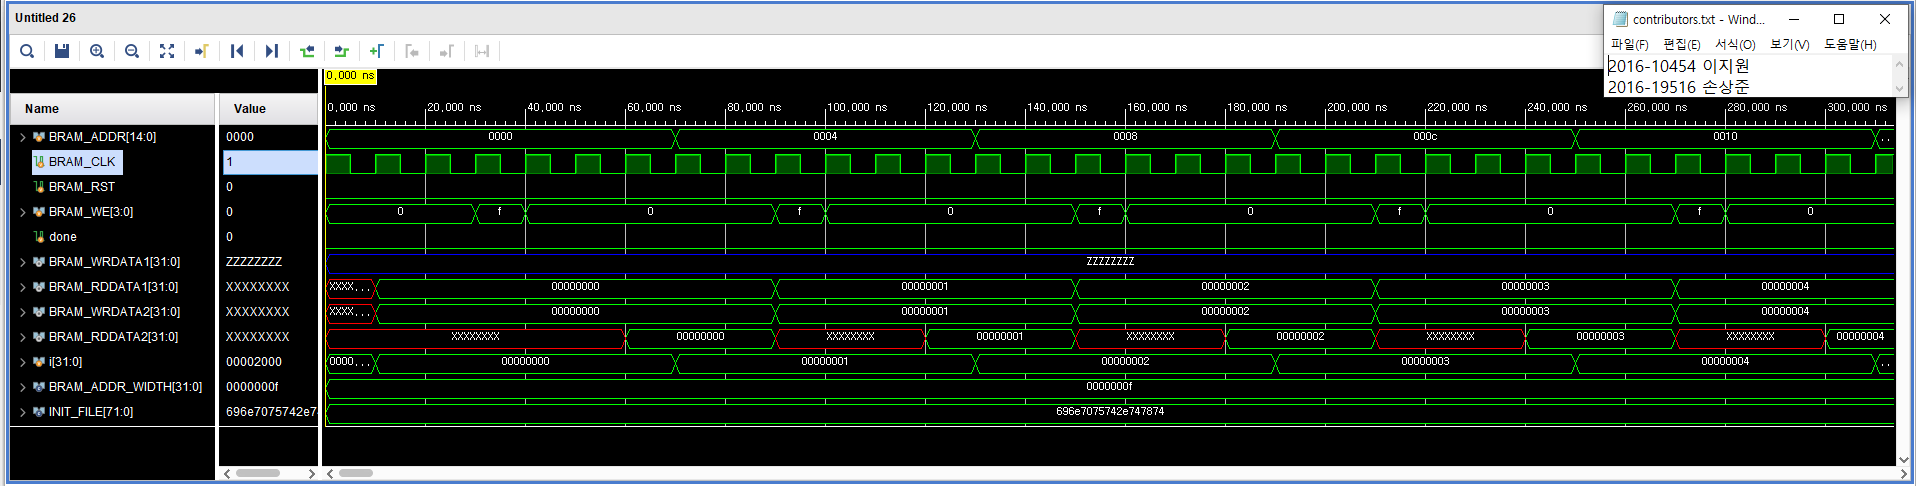
\includegraphics[width=1.0\textwidth]{../../submission/My_BRAM/My_BRAM_Waveform1.png}
	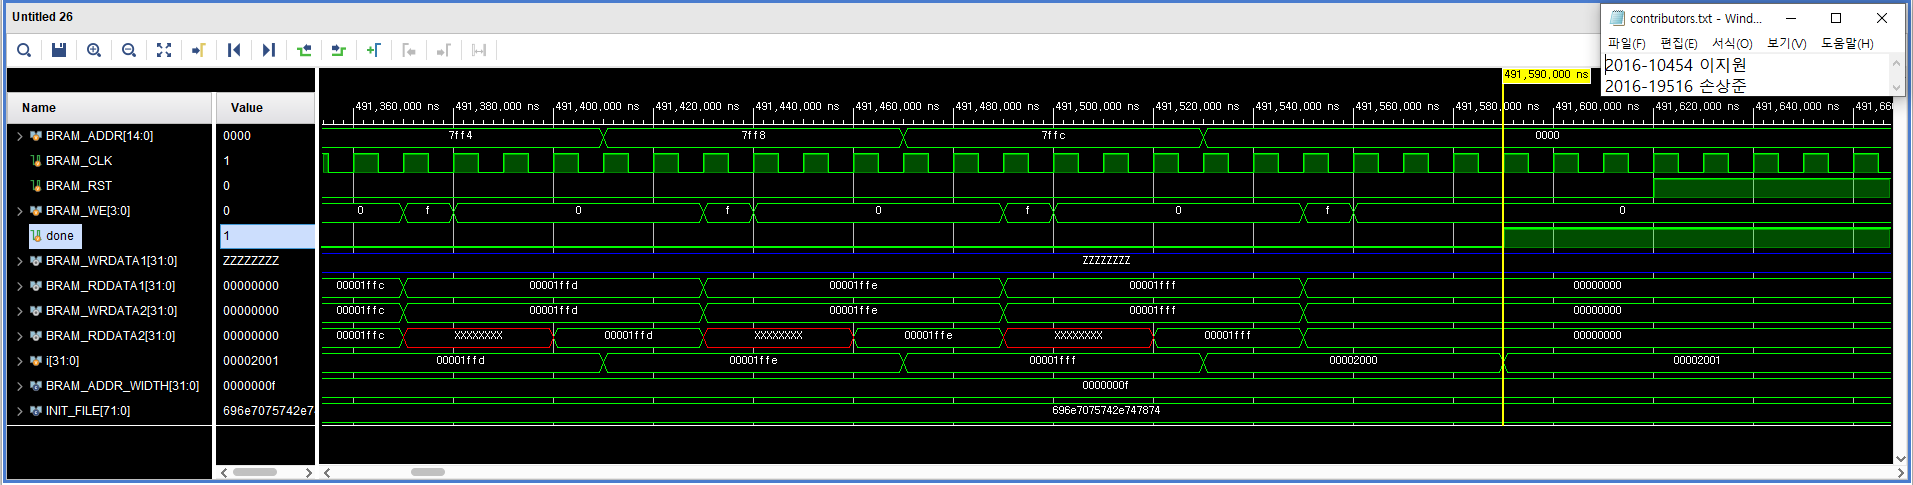
\includegraphics[width=1.0\textwidth]{../../submission/My_BRAM/My_BRAM_Waveform2.png}
\end{figure}
\begin{figure}[ht]
	\centering
	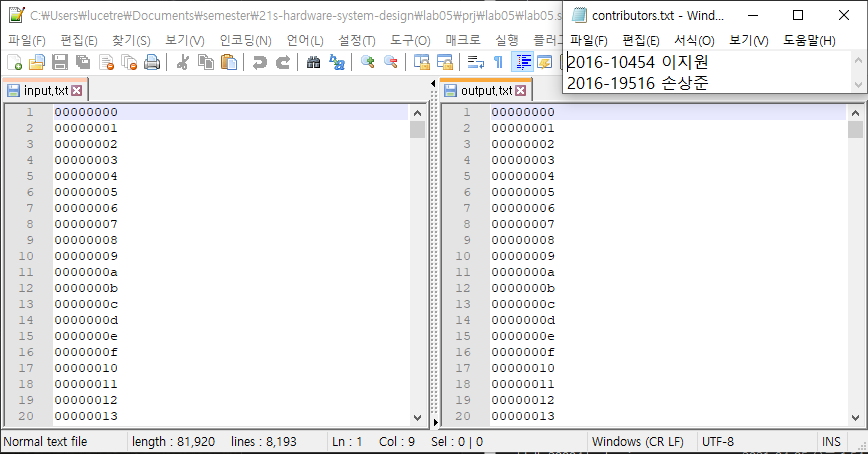
\includegraphics[width=0.8\textwidth]{../../submission/My_BRAM/My_BRAM_result.png}
\end{figure}

\subsection{Processing Element, PE}



\section{Conclusion}

입력되는 범위의 값들은 uniformly random하게 선택한 값들을 가지고 시뮬레이션 결과를 살펴보았을 때,
연산결과 값이 실제 값과 일치하는 것을 확인할 수 있었다.
Array를 이용하여 generate-for statement에서 간편하게 원하는 값을 얻어낸다는 점이 이번 프로젝트 구현 중 핵심 아이디어였다. 

cmd의 값에 따라 출력값을 변화시키기 위해 always @(cmd) 구문을 사용하지 않고, 삼항연산자를 사용할 때에도 원하는 형태로 waveform이 출력되었는데, 삼항연산자 자체도 always와 비슷한 역할로 event가 발생하면 출력값을 변화시키는 역할을 확인하였다.
향후 프로젝트에서 IP catalog를 이용해 기존의 모듈을 효율적으로 활용하여 코드를 작성하는 방법을 익힐 수 있었으며, custom modularization 과정을 익힐 수 있었다.
\newpage
\bibliographystyle{plain}
\bibliography{other}

\end{document}
